\documentclass[12pt]{article}

\usepackage{amsmath, mathtools}
\usepackage{amsfonts}
\usepackage{amssymb}
\usepackage{graphicx}
\usepackage{colortbl}
\usepackage{xr}
\usepackage{hyperref}
\usepackage{longtable}
\usepackage{xfrac}
\usepackage{tabularx}
\usepackage{float}
\usepackage{siunitx}
\usepackage{booktabs}
\usepackage{caption}
\usepackage{pdflscape}
\usepackage{afterpage}
\usepackage{amsmath} % for 'bmatrix' environment

\usepackage[round]{natbib}


%\usepackage{biblatex} --> this is incompatible with natbib
%\addbibresource{SRS.bib}

%\usepackage{refcheck}

\hypersetup{
    bookmarks=true,         % show bookmarks bar?
      colorlinks=true,       % false: boxed links; true: colored links
    linkcolor=red,          % color of internal links (change box color with linkbordercolor)
    citecolor=green,        % color of links to bibliography
    filecolor=magenta,      % color of file links
    urlcolor=cyan           % color of external links
}

%% Comments

\usepackage{color}

\newif\ifcomments\commentstrue

\ifcomments
\newcommand{\authornote}[3]{\textcolor{#1}{[#3 ---#2]}}
\newcommand{\todo}[1]{\textcolor{red}{[TODO: #1]}}
\else
\newcommand{\authornote}[3]{}
\newcommand{\todo}[1]{}
\fi

\newcommand{\wss}[1]{\authornote{blue}{SS}{#1}} 
\newcommand{\plt}[1]{\authornote{magenta}{TPLT}{#1}} %For explanation of the template
\newcommand{\an}[1]{\authornote{cyan}{Author}{#1}}

%% Common Parts

\newcommand{\progname}{ProgName} % PUT YOUR PROGRAM NAME HERE %Every program
                                % should have a name


% For easy change of table widths
\newcommand{\colZwidth}{1.0\textwidth}
\newcommand{\colAwidth}{0.13\textwidth}
\newcommand{\colBwidth}{0.82\textwidth}
\newcommand{\colCwidth}{0.1\textwidth}
\newcommand{\colDwidth}{0.05\textwidth}
\newcommand{\colEwidth}{0.8\textwidth}
\newcommand{\colFwidth}{0.17\textwidth}
\newcommand{\colGwidth}{0.5\textwidth}
\newcommand{\colHwidth}{0.28\textwidth}

% Used so that cross-references have a meaningful prefix
\newcounter{defnum} %Definition Number
\newcommand{\dthedefnum}{GD\thedefnum}
\newcommand{\dref}[1]{GD\ref{#1}}
\newcounter{datadefnum} %Datadefinition Number
\newcommand{\ddthedatadefnum}{DD\thedatadefnum}
\newcommand{\ddref}[1]{DD\ref{#1}}
\newcounter{theorynum} %Theory Number
\newcommand{\tthetheorynum}{T\thetheorynum}
\newcommand{\tref}[1]{T\ref{#1}}
\newcounter{tablenum} %Table Number
\newcommand{\tbthetablenum}{T\thetablenum}
\newcommand{\tbref}[1]{TB\ref{#1}}
\newcounter{assumpnum} %Assumption Number
\newcommand{\atheassumpnum}{P\theassumpnum}
\newcommand{\aref}[1]{A\ref{#1}}
\newcounter{goalnum} %Goal Number
\newcommand{\gthegoalnum}{P\thegoalnum}
\newcommand{\gsref}[1]{GS\ref{#1}}
\newcounter{instnum} %Instance Number
\newcommand{\itheinstnum}{IM\theinstnum}
\newcommand{\iref}[1]{IM\ref{#1}}
\newcounter{reqnum} %Requirement Number
\newcommand{\rthereqnum}{P\thereqnum}
\newcommand{\rref}[1]{R\ref{#1}}
\newcounter{lcnum} %Likely change number
\newcommand{\lthelcnum}{LC\thelcnum}
\newcommand{\lcref}[1]{LC\ref{#1}}



\usepackage{fullpage}
\renewcommand{\progname}{EEGSourceLocalization} 
\begin{document}

\title{Software Requirements Specification for \progname \ software} 
\author{Leila Mousapour}
\date{\today}
	
\maketitle

~\newpage

\pagenumbering{roman}

\tableofcontents



~\newpage

\section*{Revision History}

\begin{tabularx}{\textwidth}{p{3cm}p{2cm}X}
\toprule {\bf Date} & {\bf Version} & {\bf Notes}\\
\midrule
October 2  2020 & 1.0 & The first version\\
%Date 2 & 1.1 & Notes\\
\bottomrule
\end{tabularx}

~\newpage

\section{Reference Material}

This section records information for easy reference.

\subsection{Table of Units}

Throughout this document SI (Syst\`{e}me International d'Unit\'{e}s) is employed
as the unit system.  In addition to the basic units, several derived units are
used as described below.  For each unit, the symbol is given followed by a
description of the unit and the SI name.
~\newline

\renewcommand{\arraystretch}{1.2}
%\begin{table}[ht]
  \noindent \begin{tabular}{l l l} 
    \toprule		
    \textbf{symbol} & \textbf{unit} & \textbf{SI}\\
    \midrule 
    \si{\metre} & length & metre\\
    hz & Frequency	& herts\\
    \si{\second} & time & second\\
    \si{\volt} & voltage & volt\\
    \si{\dB} & power & Decibel \\
    \bottomrule
  \end{tabular}
  %	\caption{Provide a caption}
%\end{table}

%\plt{Only include the units that your SRS actually uses.}
%
%\plt{Derived units, like newtons, pascal, etc, should show their derivation
%    (the units they are derived from) if their constituent units are in the
%    table of units (that is, if the units they are derived from are used in the
%    document).  For instance, the derivation of pascals as
%    $\si{\pascal}=\si{\newton\per\square\meter}$ is shown if newtons and m are
%    both in the table.  The derivations of newtons would not be shown if kg and
%    s are not both in the table.}
%
%\plt{The symbol for units named after people use capital letters, but the name
%  of the unit itself uses lower case.  For instance, pascals use the symbol Pa,
%  watts use the symbol W, teslas use the symbol T, newtons use the symbol N,
%  etc.  The one exception to this is degree Celsius.  Details on writing metric
%  units can be found on the 
%  \href{https://www.nist.gov/pml/weights-and-measures/writing-metric-units}
%  {NIST} web-page.}
%
%\subsection{Table of Symbols}
%
%The table that follows summarizes the symbols used in this document along with
%their units. The symbols are listed in alphabetical order.
%
%\renewcommand{\arraystretch}{1.2}
%%\noindent \begin{tabularx}{1.0\textwidth}{l l X}
%\noindent \begin{longtable*}{l l p{12cm}} \toprule
%\textbf{symbol} & \textbf{unit} & \textbf{description}\\
%\midrule 
%$A_C$ & \si[per-mode=symbol] {\square\metre} & coil surface area
%\\
%$A_\text{in}$ & \si[per-mode=symbol] {\square\metre} & surface area over 
%which heat is transferred in
%\\ 
%\bottomrule
%\end{longtable*}
%\plt{Use your problems actual symbols.  The si package is a good idea to use for
%  units.}

\subsection{Abbreviations and Acronyms}

\renewcommand{\arraystretch}{1.2}
\begin{tabular}{l l} 
  \toprule		
  \textbf{symbol} & \textbf{description}\\
  \midrule 
  A & Assumption\\
  DD & Data Definition\\
  GD & General Definition\\
  GS & Goal Statement\\
  IM & Instance Model\\
  LC & Likely Change\\
  PS & Physical System Description\\
  R & Requirement\\
  SRS & Software Requirements Specification\\
 EEGSourceLocalizer & Electroencephalogram Source Localization Software\\ %\plt{put an expanded version of your program name here (as appropriate)}\\
  T & Theoretical Model\\
  EEG & Electroencephalogram \\
  BCI & Brain-Computer Interface\\
  SL & Source Localization \\
  ML & Machine Learning \\
  LCMV & Linearly Constraint Minimum Variance \\
  DICS & Dynamic Imaging of Coherent Sources\\

  \bottomrule
\end{tabular}\\

%\plt{Add any other abbreviations or acronyms that you add}

%\newpage

\pagenumbering{arabic}

%\plt{This SRS template is based on \citet{SmithAndLai2005, SmithEtAl2007}.  It
%  will get you started.  You should not modify the section headings, without
%  first discussing the change with the course instructor.  Modification means
%  you are not following the template, which loses some of the advantage of a
%  template, especially standardization.  Although the bits shown below do not
%  include type information, you may need to add this information for your
%  problem.  If you are unsure, please can ask the instructor.}
%
%\plt{Feel free to change the appearance of the report by modifying the LaTeX
%  commands.}
%
%\plt{This template document assumes that a single program is being documented.
%  If you are documenting a family of models, you should start with a commonality
%  analysis.  A separate template is provided for this.  For program
%  families you should look at \cite{Smith2006, SmithMcCutchanAndCarette2017}.
%  Single family member programs are often programs based on a single physical
%  model.  General purpose tools are usually documented as a family.  Families of
%  physical models also come up.}
%
%\plt{The SRS is not generally written, or read, sequentially.  The SRS is a
%  reference document.  It is generally read in an ad hoc order, as the need
%  arises.  For writing an SRS, and for reading one for the first time, the
%  suggested order of sections is:
%\begin{itemize}
%\item Goal Statement
%\item Instance Models
%\item Requirements
%\item Introduction
%\item Specific System Description
%\end{itemize}
%}
%
%\plt{Guiding principles for the SRS document:
%\begin{itemize}
%\item Do not repeat the same information at the same abstraction level.  If
%  information is repeated, the repetition should be at a different abstraction
%  level.  For instance, there will be overlap between the scope section and the
%  assumptions, but the scope section will not go into as much detail as the
%  assumptions section.
%\end{itemize}
%}
%
%\plt{The template description comments should be disabled before submitting this
%  document for grading.}
%
%\plt{You can borrow any wording from the text given in the template.  It is part
%  of the template, and not considered an instance of academic integrity.  Of
%  course, you need to cite the source of the template.}
%
%\plt{When the documentation is done, it should be possible to trace back to the
%  source of every piece of information.  Some information will come from
%  external sources, like terminology.  Other information will be derived, like
%  General Definitions.}
%
%\plt{An SRS document should have the following qualities: unambiguous,
%  consistent, complete, validatable, abstract and traceable.}
%
%\plt{The overall goal of the SRS is that someone that meets the Characteristics
%  of the Intended Reader (Section~\ref{sec_IntendedReader}) can learn,
%  understand and verify the captured domain knowledge.  They should not have to
%  trust the authors of the SRS on any statements.  They should be able to
%  independently verify/derive every statement made.}

\section{Introduction}
Electroencephalography (EEG), which is a method to record electrical activity of the brain, has a plethora of applications such as decoding mental imageries used in brain-computer interfaces (BCI). One of the big open problems in EEG signal processing is finding a good feature space after which we can apply machine learning and classification methods to the data. The standard in the field is to start with the electrode space and then extract features such as amplitude or latencies (time domain features), frequency power spectra (frequency features), common spatial patterns (spatial features) etc. A novel approach that we would like to investigate is to first map EEG signals from electrode space into spatial coordinates of the brain to achieve more useful features \cite{michel_eeg_2019}.\\

These techniques are known as “source localization “ algorithms which can be applied to the signals recorded from the scalp and locate the underlying active sources generating the activity sensed on the electrodes expected to increase the signal to noise ratio. Additionally, mapping the activity from an n-channel space to fewer sources reduces data dimensionality immensely, helps avoid overfitting and redundancy, leads to better human interpretations and less computational cost with the simplification of models. Therefore, this scientific software aims to implement several techniques to map EEG signals from electrode space to source space.\\

In this introduction, first the purpose of the SRS document is discussed. Afterwards, the scope of requirements for the software are stated from the big picture view. Additionally, the required skills and knowledge for the readers of this document are clarified. This section will end by illustrating a road map of the whole SRS document.

%  SRS.his section summarizes the skills and knowledge of the readers of the
%  SRS.Finally, 

%\plt{The introduction section is written to introduce the problem.  It starts
%  general and focuses on the problem domain. The general advice is to start with
%a paragraph or two that describes the problem, followed by a ``roadmap''
%paragraph.  A roadmap orients the reader by telling them what sub-sections to
%expect in the Introduction section.}

\subsection{Purpose of Document}
This main purpose of this document is to explain the modelling of an EEG source localization system and describes the features and behaviours of the \progname{}  software application. It includes a variety of elements that attempts to define the intended functionality required by the user. Thus, this document provides detailed requirements of the software which will be used in planing for design stage. Therefore, this document is intended to be used as a reference to provide ad hoc access to all information necessary to understand and verify the model. \

Goals, assumptions, theoretical models, definitions, and other model derivation information are explained, allowing the reader to fully understand and verify the purpose and scientific basis of EEGSourceLocalizer. This SRS will remain abstract, describing what problem is being solved, but not how to solve it. This document, which fits in a series of documents that follow the so-called waterfall model, will be used as a starting point for subsequent development phases, including writing the design specification and the software verification and validation plan \cite{Parnas1978}.

%\plt{This section summarizes the purpose of the SRS document.  It does not focus
%  on the problem itself.  The problem is described in the ``Problem
%  Description'' section (Section~\ref{Sec_pd}).  The purpose is for the document
%  in the context of the project itself, not in the context of the CAS 741
%  course.  Although the ``purpose'' of the document is to get a grade in 741,
%  you should not mention this.  Instead, ``fake it'' as if this is a real
%  project.  The purpose section will be similar between projects.  The purpose
%  of the document is the purpose of the SRS, including communication, planning
%  for the design stage, etc.}

\subsection{Scope of Requirements} 

Source localization is a very general problem which can be in raised in various contexts such as telecommunication signals, sound signals, brain signals etc. Also, there are numerous algorithms with different set of assumptions to solve this problem. However, the scope of the requirements for this project is limited to source localization of EEG signals and it will not be applicable to other neuroimaging modalities such as magnetoencephalggram (MEG), fNIRS etc. Moreover, this software will only use 2 different algorithms of source localization: Beamforming (LCMV) and sLORETA and will not cover other approaches.

%\plt{Modelling the real world requires simplification.  The full complexity of
%  the actual physics, chemistry, biology is too much for existing models, and
%  for existing computational solution techniques.  Rather than say what is in
%  the scope, it is usually easier to say what is not.  You can think of it as
%  the scope is initially everything, and then it is constrained to create the
%  actual scope.  For instance, the problem can be restricted to 2 dimensions, or
%  it can ignore the effect of temperature (or pressure) on the material
%  properties, etc.}  

%\plt{The scope section is related to the assumptions section
%  (Section~\ref{sec_assumpt}).  However, the scope and the assumptions are not
%  at the same level of abstraction.  The scope is at a high level.  The focus is
%  on the ``big picture'' assumptions.  The assumptions section lists, and
%  describes, all of the assumptions.}

\subsection{Characteristics of Intended Reader} \label{sec_IntendedReader}

The intended readers are the people who will read, review and maintain the SRS.  They are the people that will conceivably design the software that is intended to meet the requirements. Therefore, they are expected to have a general understanding of EEG neuroimaging technique and EEG signal processing. Also, a very good knowledge of linear algebra and matrix manipulation is required to understand the modelling of the SL problem. 

%\plt{This section summarizes the skills and knowledge of the readers of the
%  SRS.  It does NOT have the same purpose as the ``User Characteristics''
%  section (Section~\ref{SecUserCharacteristics}).  The intended readers are the
%  people that will read, review and maintain the SRS.  They are the people that
%  will conceivably design the software that is intended to meet the
%  requirements.  The user, on the other hand, is the person that uses the
%  software that is built.  They may never read this SRS document.  Of course,
%  the same person could be a ``user'' and an ``intended reader.''}
%
%\plt{The intended reader characteristics should be written as unambiguously and
%  as specifically as possible.  Rather than say, the user should have an
%  understanding of physics, say what kind of physics and at what level.  For
%  instance, is high school physics adequate, or should the reader have had a
%  graduate course on advanced quantum mechanics?}

\subsection{Organization of Document}

The document follows the organizational scheme for an SRS for scientific computing software  laid out by Smith \textit{et al.}
\cite{SmithAndLai2005}, starting with general reference
material for the reader. The introduction of the document details the purpose of
the document and qualifications of the intended reader, and is followed by the General System Description. The Specific System Description elaborates on the problem and defines needed terminology. Afterwards, the goal statements  of the \progname{} are listed which are refined to the theoretical models, and the theoretical models to the instance models to explain to solution characteristics. The
Requirements section of the document clearly outlines both the Functional and
Non-functional Requirements that the software must comply with. Finally, the
document contains a list of Likely Changes to the software and Traceability
matrices and graphs.

\newpage
%\plt{This section provides a roadmap of the SRS document.  It will help the
%  reader orient themselves.  It will provide direction that will help them
%  select which sections they want to read, and in what order.  This section will
%  be similar between project.}

\section{General System Description}

This section provides general information about the system.  It identifies the
interfaces between the system and its environment, describes the user
characteristics and lists the system constraints.  
%\plt{This text can likely be
%  borrowed verbatim.}
%
%\plt{The purpose of this section is to provide general information about the
%  system so the specific requirements in the next section will be easier to
%  understand. The general system description section is designed to be
%  changeable independent of changes to the functional requirements documented in
%  the specific system description. The general system description provides a
%  context for a family of related models.  The general description can stay the
%  same, while specific details are changed between family members.}

\subsection{System Context}


Figure \ref{Fig_SystemContext} shows the system context which is an abstract view of the software. A circle represents an external entity outside the software, the user in this case. A rectangle represents the software system itself (EEGSourceLocalizer). Arrows are used to show the data flow between the system and its environment including the main inputs and outputs. The responsibilities of the user and the system are as follows:

%\plt{Your system context will include a figure that shows the abstract view of
%  the software.  Often in a scientific context, the program can be viewed
%  abstractly following the design pattern of Inputs $\rightarrow$ Calculations
%  $\rightarrow$ Outputs.  The system context will therefore often follow this
%  pattern.  The user provides inputs, the system does the calculations, and then
%  provides the outputs to the user.  The figure should not show all of the
%  inputs, just an abstract view of the main categories of inputs (like material
%  properties, geometry, etc.).  Likewise, the outputs should be presented from
%  an abstract point of view.  In some cases the diagram will show other external
%  entities, besides the user.  For instance, when the software product is a
%  library, the user will be another software program, not an actual end user.}

\begin{figure}[h!]
\begin{center}
 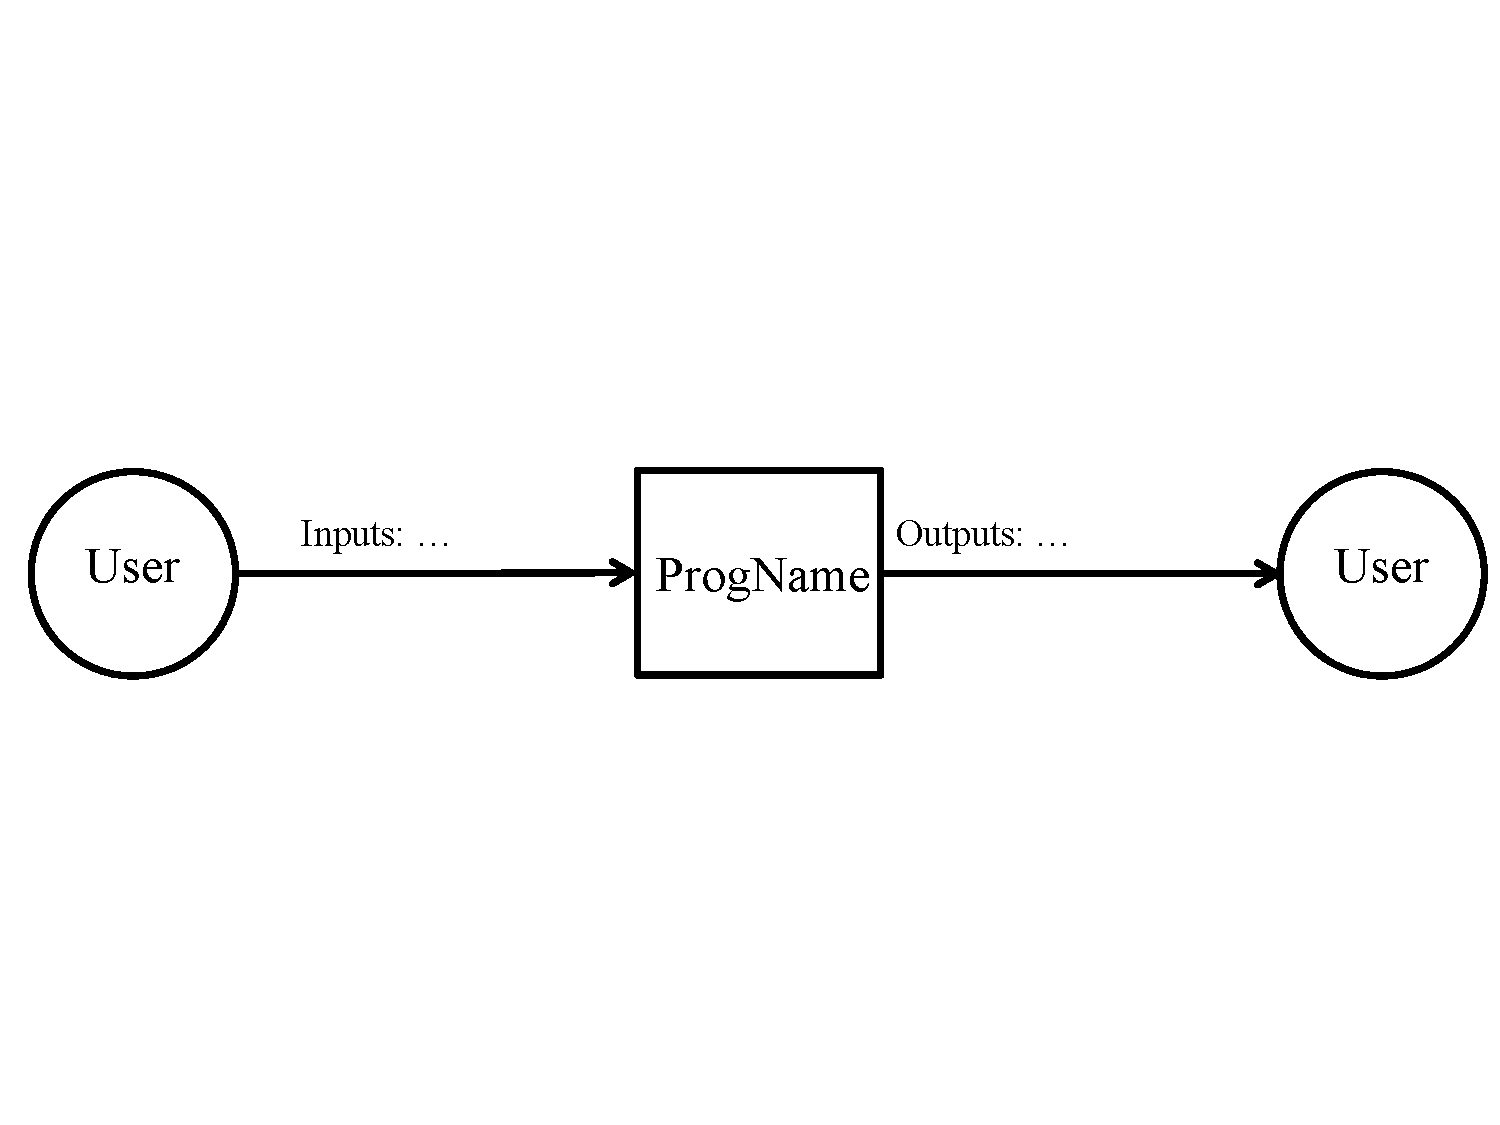
\includegraphics[width=0.6\textwidth]{SystemContextFigure}
\caption{System Context}
\label{Fig_SystemContext} 
\end{center}
\end{figure}

%\plt{For each of the entities in the system context diagram its responsibilities
%  should be listed.  Whenever possible the system should check for data quality,
%  but for some cases the user will need to assume that responsibility.}

\begin{itemize}
\item User Responsibilities:
\begin{itemize} 
\item  Clean and preprocess the EEG data (remove artifacts as it adversely affects the SL accuracy)
\item  Provide all the input data to the system (including EEG recording and electrode location file) 
\item  Given two or more options by the system, decide which SL method to use
\end{itemize}

\item \progname{} Responsibilities:
\begin{itemize}
\item Detect data type mismatch or missing inputs
\item Determine if the inputs satisfy the required physical and software constraints
\item Calculate and plot the required outputs
\end{itemize}
\end{itemize}

\subsection{User Characteristics} \label{SecUserCharacteristics}

The user is expected to be familiar with EEG cleaning and preprocessing to provide the software with cleaned data such as artifact removal as SL techniques are very sensitive to the data quality. Also, the user should have the knowledge about the different techniques that are provided as SL options in this software to be able to set the configurations of the methods. For this purpose, they should have an understanding of signal processing and linear algebra. Additionally, the end user is preferred to have a basic cognitive neuroscience knowledge so that they have a rough idea where  to expect the active sources during the task performed by the participant.

%\plt{This section summarizes the knowledge/skills expected of the user.
%  Measuring usability, which is often a required non-function requirement,
%  requires knowledge of a typical user.  As mentioned above, the user is a
%  different role from the ``intended reader,'' as given in
%  Section~\ref{sec_IntendedReader}.  As in Section~\ref{sec_IntendedReader}, the
%  user characteristics should be specific an unambiguous.  For instance, ``The
%  end user of \progname{} should have an understanding of undergraduate Level 1
%  Calculus and Physics.''}

\subsection{System Constraints}

There is no system constraints for this project.


%\plt{System constraints differ from other type of requirements because they
%  limit the developers’ options in the system design and they identify how the
%  eventual system must fit into the world. This is the only place in the SRS
%  where design decisions can be specified.  That is, the quality requirement for
%  abstraction is relaxed here.  However, system constraints should only be
%  included if they are truly required. In the context of CAS 741, you often will
%  may not have any system constraints.}

\newpage 
\section{Specific System Description}

This section first presents the problem description, which gives a high-level
view of the problem to be solved.  This is followed by the solution characteristics
specification, which presents the assumptions, theories, definitions and finally
the instance models.  
%\plt{Add any project specific details that are relevant
%  for the section overview.}

\subsection{Problem Description} \label{Sec_pd}

During the rest state or while performing any physical or mental task, there are many activities occurring inside the brain which we can record a superficial effect of them sensed on the scalp via EEG electrodes. However, different parts of the brain have different functionalities and their level and pattern of activity varies while performing specific tasks. \progname{} is intended to estimate the activity of the underlying sources responsible for the electric potentials record from the scalp.
%\plt{What problem does your program solve?
%The description here should be in the problem space, not the solution space.}

\subsubsection{Terminology and  Definitions}

%\plt{This section is expressed in words, not with equations.  It provide the
%  meaning of the different words and phrases used in the domain of the problem.
%The terminology is used to introduce concepts from the world outside of the
%mathematical model  The terminology provides a real world connection to give the
%mathematical model meaning.}

This subsection provides a list of terms that are used in the subsequent
sections and their meaning, with the purpose of reducing ambiguity and making it
easier to correctly understand the requirements:

\begin{itemize} 

\item EEG : The electroencephalogram (EEG) is a recording of the electrical activity of the brain from the scalp. The recorded waveforms reflect the cortical electrical activity. Signal intensity: EEG activity is quite small, measured in microvolts.

\item MRI: Magnetic resonance imaging (MRI) is a medical imaging technique that uses a magnetic field and computer-generated radio waves to create detailed images of the organs and tissues in your body.

\item Tissue conductivity: A constant describing the electrical conductivity of different head tissues.  While modelling the head, we have to consider the electrical conductivity of the different head tissues (brain, skull, scalp) are different. 

\item Coordinate system: in geometry, a coordinate system is a system that uses one or more numbers, or coordinates, to uniquely determine the position of the points or other geometric elements on a manifold such as Euclidean space.

\item Covariance: In probability theory and statistics, a covariance matrix is a square matrix giving the covariance between each pair of elements of a given random vector.

\item Rank: The maximum number of linearly independent vectors in a matrix is equal to the number of non-zero rows in its row echelon matrix. Therefore, to find the rank of a matrix, we simply transform the matrix to its row echelon form and count the number of non-zero rows.

\item Rank-deficient: A matrix is said to be rank-deficient if it does not have full rank. The rank deficiency of a matrix is the difference between the lesser between the number of rows and columns, and the rank.

\item Beamforming:  Beamforming or spatial filtering is a signal processing technique used in sensor arrays for directional signal transmission or reception.

\end{itemize}

\subsubsection{Physical System Description} \label{sec_phySystDescrip}

The purpose of this section is to clearly and unambiguously state the physical system that is to be modelled. The complete physical system consist of two main components: the head and the EEG equipments (electrodes) placed on the the scalp. Each of these 2 have several elements. \\

EEG equipment consist of a number of electrodes (could be anything between 6 to 256 electrodes) placed on predefined locations. These locations could be specified by a cap or by sectioning the head. Also, head can be physically modeled with 3 tissues with different conductivity: brain, skull and scalp.  \\

%\plt{The purpose of this section is to clearly and unambiguously state the
%  physical system that is to be modelled. Effective problem solving requires a
%  logical and organized approach. The statements on the physical system to be
%  studied should cover enough information to solve the problem. The physical
%  description involves element identification, where elements are defined as
%  independent and separable items of the physical system. Some example elements
%  include acceleration due to gravity, the mass of an object, and the size and
%  shape of an object. Each element should be identified and labelled, with their
%  interesting properties specified clearly. The physical description can also
%  include interactions of the elements, such as the following: i) the
%  interactions between the elements and their physical environment; ii) the
%  interactions between elements; and, iii) the initial or boundary conditions.}

The physical system of \progname{}, as shown in Figure \ref{Fig_PhysicalSystem} ,
includes the following elements:

\begin{itemize}

\item[PS1:] EEG recording electrodes
\item[PS2:] Head (Scull, scalp and brain)

\end{itemize}

%\plt{A figure here makes sense for most SRS documents}

\begin{figure}[h!]
\begin{center}
 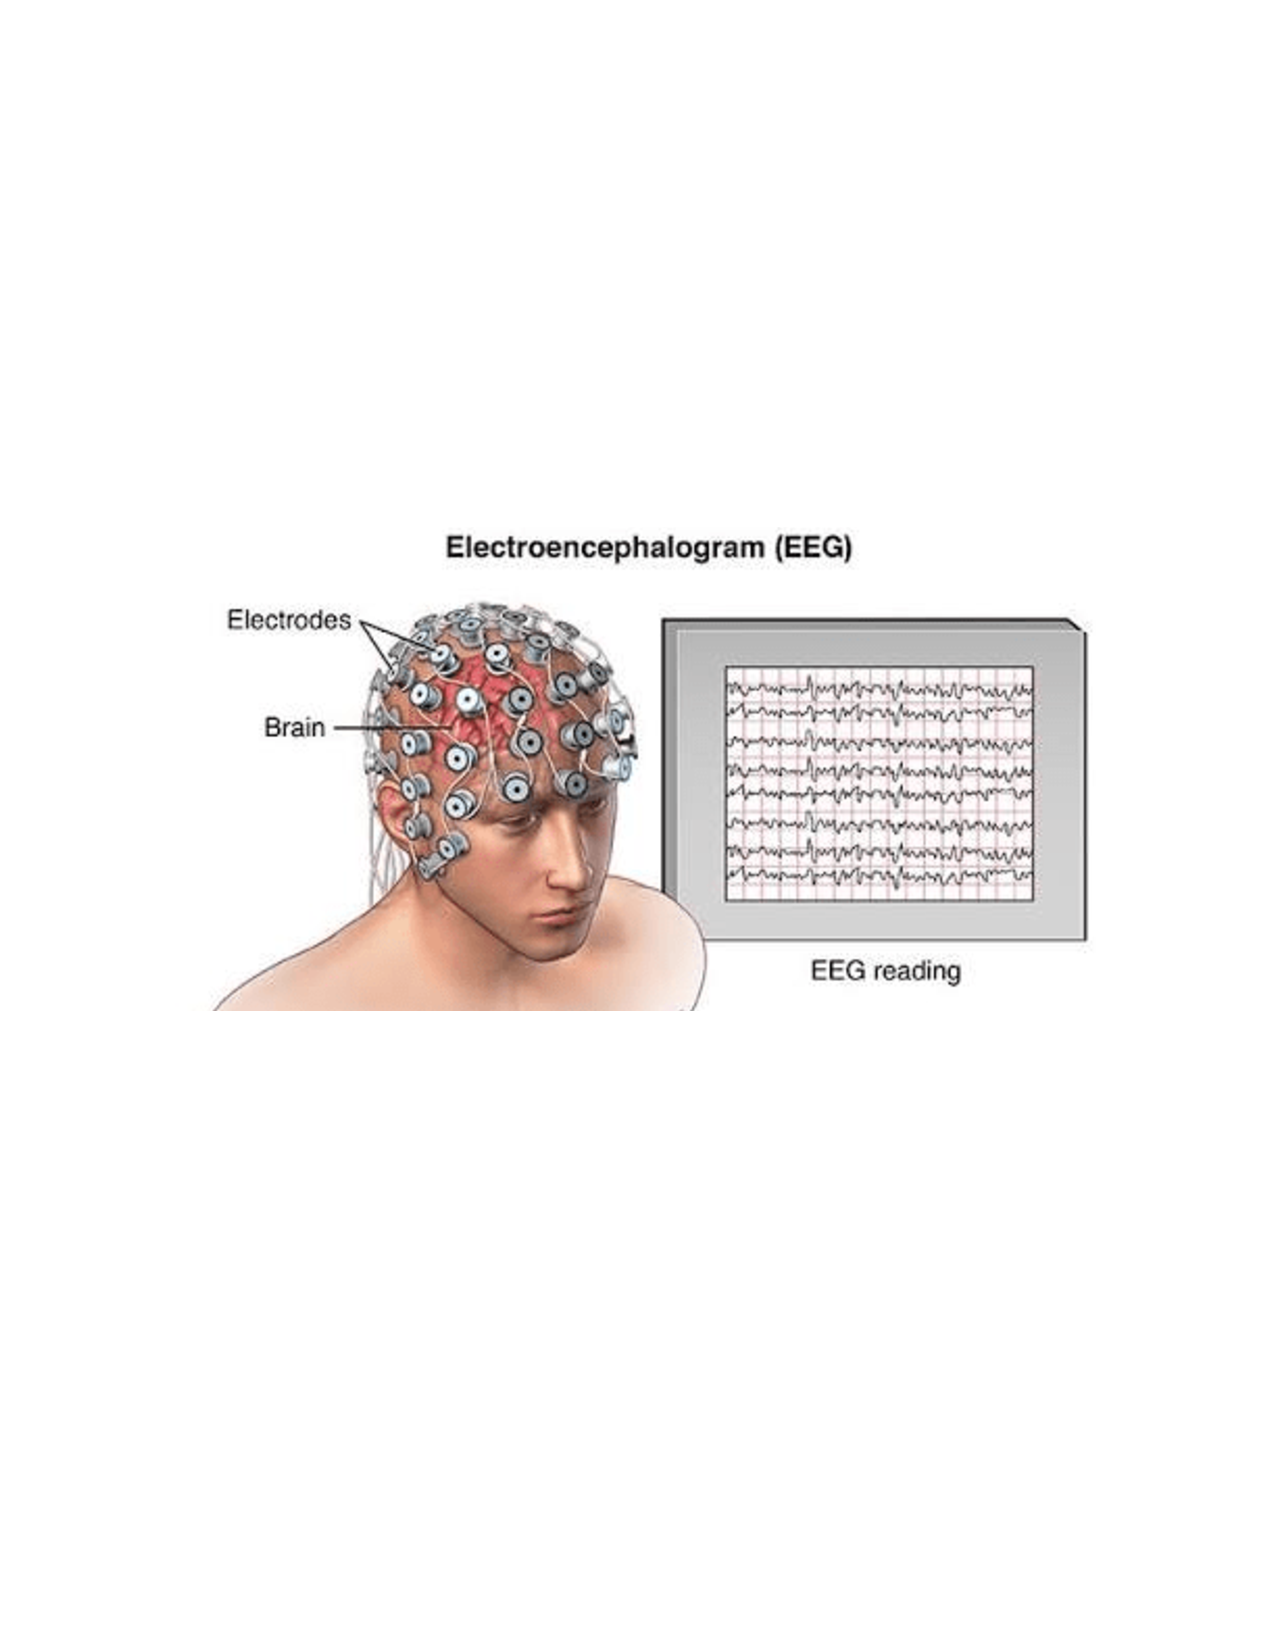
\includegraphics[width=0.6\textwidth]{EEG-recording}
\caption{Physical System Schematic}
\label{Fig_PhysicalSystem}
\end{center}
\end{figure}

% \begin{figure}[h!]
% \begin{center}
% %\rotatebox{-90}
% {
%  \includegraphics[width=0.5\textwidth]{<FigureName>}
% }
% \caption{\label{<Label>} <Caption>}
% \end{center}
% \end{figure}

\newpage

\subsubsection{Goal Statements}

%\plt{The goal statements refine the ``Problem Description''
%  (Section~\ref{Sec_pd}).  A goal is a functional objective the system under
%  consideration should achieve. Goals provide criteria for sufficient
%  completeness of a requirements specification and for requirements
%  pertinence. Goals will be refined in Section “Instanced Models”
%  (Section~\ref{sec_instance}). Large and complex goals should be decomposed
%  into smaller sub-goals.  The goals are written abstractly, with a minimal
%  amount of technical language.  They should be understandable by non-domain
%  experts.}

\noindent Given the inputs including the recorded EEG signal, the location of electrodes in appropriate coordination system, the head MRI and the choice of SL algorithm, the goal statements are:

\begin{itemize}

\item[GS\refstepcounter{goalnum}\thegoalnum \label{G_meaningfulLabel}:] Create a source model by segmenting the brain volume or the cortical surface into voxels (brain mesh grid)\item[GS\refstepcounter{goalnum}\thegoalnum \label{G_meaningfulLabel}:] Estimate the sources activity in time (source time course) for every source point in the generated source model
\item[GS\refstepcounter{goalnum}\thegoalnum \label{G_meaningfulLabel}:] Estimate the average source power (over time) for all source points
\item[GS\refstepcounter{goalnum}\thegoalnum \label{G_meaningfulLabel}:] Plot the sources on a sliced MRI or 3D brain model 


%\plt{One
%    sentence description of the goal.  There may be more than one.  Each Goal
%    should have a meaningful label.}
%    
    

\end{itemize}

\subsection{Solution Characteristics Specification}
This section specifies the information in the solution domain of the system
to be developed and is intended to express what is required in
such a way that analysts and stakeholders get a clear picture, and the
latter will accept it. The purpose of this section is to reduce the problem into one expressed in mathematical terms.\\

This section presents the solution characteristics by successively refining
models. It starts with the abstract/general Theoretical Models (TMs) and
refines them to the concrete/specific Instance Models (IMs). All of these
refinements can potentially use Assumptions (A) and Data Definitions (DD). DDs are not refined; they are just used. GDs and IMs are derived, or refined, from other
models. DDs are not derived; they are just given. TMs are also just given, but
they are refined, not used.  Figure \ref{Fig_SolChar} shows the relation between these subsections\\


%\plt{This section specifies the information in the solution domain of the system
%  to be developed. This section is intended to express what is required in
%  such a way that analysts and stakeholders get a clear picture, and the
%  latter will accept it. The purpose of this section is to reduce the problem
%  into one expressed in mathematical terms. Mathematical expertise is used to
%  extract the essentials from the underlying physical description of the
%  problem, and to collect and substantiate all physical data pertinent to the
%  problem.}
%
%\plt{This section presents the solution characteristics by successively refining
%  models.  It starts with the abstract/general Theoretical Models (TMs) and
%  refines them to the concrete/specific Instance Models (IMs).  If necessary
%  there are intermediate refinements to General Definitions (GDs).  All of these
%  refinements can potentially use Assumptions (A) and Data Definitions (DD).
%  TMs are refined to create new models, that are called GMs or IMs. DDs are not
%  refined; they are just used. GDs and IMs are derived, or refined, from other
%  models. DDs are not derived; they are just given. TMs are also just given, but
%  they are refined, not used.  If a potential DD includes a derivation, then
%  that means it is refining other models, which would make it a GD or an IM.}
%
%\plt{The above makes a distinction between ``refined'' and ``used.'' A model is
%  refined to another model if it is changed by the refinement. When we change a
%  general 3D equation to a 2D equation, we are making a refinement, by applying
%  the assumption that the third dimension does not matter. If we use a
%  definition, like the definition of density, we aren't refining, or changing
%  that definition, we are just using it.}
%
%\plt{The same information can be a TM in one problem and a DD in another.  It is
%  about how the information is used.  In one problem the definition of
%  acceleration can be a TM, in another it would be a DD.}
%
%\plt{There is repetition between the information given in the different chunks
%  (TM, GDs etc) with other information in the document.  For instance, the
%  meaning of the symbols, the units etc are repeated.  This is so that the
%  chunks can stand on their own when being read by a reviewer/user.  It also
%  facilitates reuse of the models in a different context.}
%
%\noindent \plt{The relationships between the parts of the document are show in
%  the following figure.  In this diagram ``may ref'' has the same role as
%  ``uses'' above.  The figure adds ``Likely Changes,'' which are able to
%  reference (use) Assumptions.}

\begin{figure}[H]
  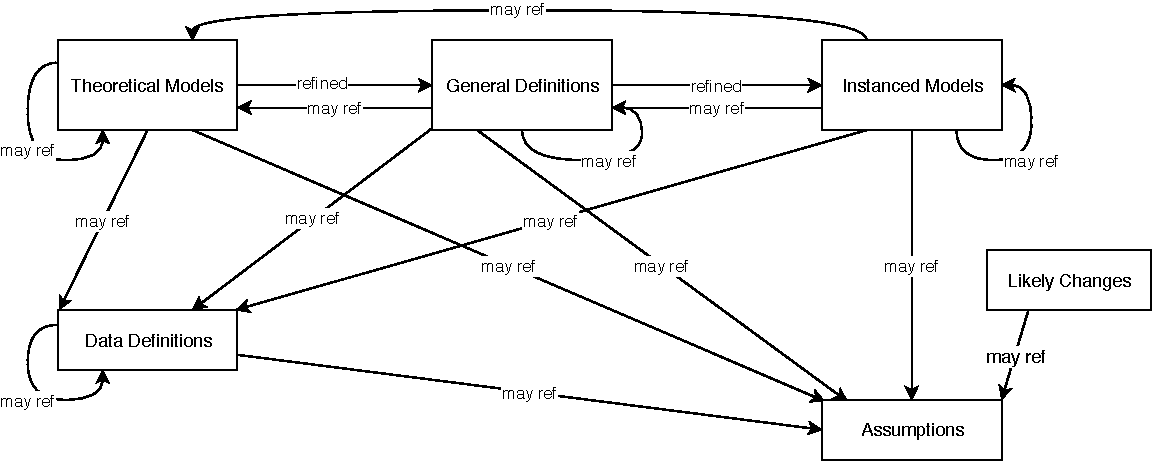
\includegraphics[scale=0.9]{RelationsBetweenTM_GD_IM_DD_A.pdf}
  \caption{Solution Characteristics Specification Subsections}
\label{Fig_SolChar}
\end{figure}


\subsubsection{Assumptions} \label{sec_assumpt}

%\plt{The assumptions are a refinement of the scope.  The scope is general, where
%  the assumptions are specific.  All assumptions should be listed, even those
%  that domain experts know so well that they are rarely (if ever) written down.}
%\plt{The document should not take for granted that the reader knows which
%  assumptions have been made. In the case of unusual assumptions, it is
%  recommended that the documentation either include, or point to, an explanation
%  and justification for the assumption.}

This section simplifies the original problem and helps in developing the
theoretical model by filling in the missing information for the physical
system. The numbers given in the square brackets refer to the theoretical model
[T], data definition [DD], instance model [IM], or
likely change [LC], in which the respective assumption is used.

\begin{itemize}

\item[A\refstepcounter{assumpnum}\theassumpnum \label{A_CD}:]
Each source is a current dipole [\tref{T_CurrentDipole}].
\item[A\refstepcounter{assumpnum}\theassumpnum \label{A_BrainOnly}:]
Sources of activity recorded in EEG are from the brain and there is no active source outside of the brain volume (meaning that we assume the eye movemnet and other muscle artifacts are rejected and only the activity from the brain is present in the EEG) [\tref{T_FP}, \tref{T_IP}].
\item[A\refstepcounter{assumpnum}\theassumpnum \label{A_AllChan}:]
Every current source contributes to ALL the channels [\tref{T_FP}, \tref{T_IP}].
\item[A\refstepcounter{assumpnum}\theassumpnum \label{A_SP}:] The activity at each channel is a linear combination of ALL sources' activities (superposition of the sensed activity of all sources at that channel) (we base the forward problem modelling on this)  [\tref{T_FP}, \tref{T_IP}].
\item[A\refstepcounter{assumpnum}\theassumpnum \label{A_SufData}:]Sufficient length of stationary data (only related to the function of interest) to get a good estimate of covariance matrix [\tref{T_IP}].
\item[A\refstepcounter{assumpnum}\theassumpnum \label{A_TC}:] The tissue conductivity is constant across each tissue type  [\iref{IM_HM}].
\item[A\refstepcounter{assumpnum}\theassumpnum \label{A_alg}:]  This software will only implement LCMV and sLORETA [\iref{IM_LCMV}].

%  \plt{Short description of each assumption.  Each assumption
%    should have a meaningful label.  Use cross-references to identify the
%    appropriate traceability to T, GD, DD etc., using commands like dref, ddref
%    etc.  Each assumption should be atomic - that is, there should not be an
%    explicit (or implicit) ``and'' in the text of an assumption.}

\end{itemize}

\newpage
\subsubsection{Theoretical Models}\label{sec_theoretical}

%\plt{Theoretical models are sets of abstract mathematical equations or axioms
%  for solving the problem described in Section ``Physical System Description''
%  (Section~\ref{sec_phySystDescrip}). Examples of theoretical models are
%  physical laws, constitutive equations, relevant conversion factors, etc.}

This section focuses on the general equations and laws that \progname{} is based on. Theoretical models are sets of abstract mathematical equations or axioms for solving the problem described in Section ``Physical System Description''. The fundamental idea of source localization is divided into two main problems: one is termed a forward problem and the other is an inverse problem. The forward problem is the prediction of potential differences from the current sources inside the brain, and the estimation of the location of the sources from the measured data is termed as inverse problem.%  \plt{Modify the examples below for your problem, and add additional models
%  as appropriate.}

~\newline

\noindent
\begin{minipage}{\textwidth}
\renewcommand*{\arraystretch}{1.5}
\begin{tabular}{| p{\colAwidth} | p{\colBwidth}|}
  \hline
  \rowcolor[gray]{0.9}
  Number& T\refstepcounter{theorynum}\thetheorynum \label{T_CurrentDipole}\\
  \hline
  Label&\bf Current Dipole\\
  \hline
  Equation&  $d$ = $\mathbf{I} p n'_d$\\
  \hline
  Description & 
	 The electrical activity inside the brain can be modeled as a current dipole. This dipole provides good approximation for a small source viewed from a relatively large distance, as the far field of a realistic source is mainly dipolar.\\ 
	& The current dipole consists of the current source and the sink separated by distance $p$ with an equal amount of current to be injected or removed. The magnitude and orientation of dipole are characterized by the dipole moment $d$ vector, which is pointing from the source to the sink in the figure. Hence, the magnitude of the dipole is $|d|= \mathbf{I} p$, where $p$ is the distance between the positive and negative poles, respectively. $n'$ is the unit vector defining the direction from the source to the $d$ sink. However, in the Cartesian coordinate system, the dipole can be represented by $x ,y, z$ unit vectors (\aref{A_CD}).\\
  \hline
  Source &
           Jatoi, M. A. (2019). Brain Source Localization Using EEG Signal Analysis. CRC Press.\\
  % The above web link should be replaced with a proper citation to a publication
  \hline
  Ref.\ By & \iref{IM_LF}\\
  \hline
\end{tabular}
\end{minipage}\\


~\newline

\noindent
\begin{minipage}{\textwidth}
\renewcommand*{\arraystretch}{1.5}
\begin{tabular}{| p{\colAwidth} | p{\colBwidth}|}
  \hline
  \rowcolor[gray]{0.9}
  Number& T\refstepcounter{theorynum}\thetheorynum \label{T_FP}\\
  \hline
  Label&\bf Forward Problem/Model\\
  \hline
  Equation&  $x$ = $\sum_{i=1}^{L} \mathbf{H(q_i) m(q_i)} + n$\\
  \hline
  Description & 
                The forward problem is concerned with the computation of scalp potentials for a specific set of neural current sources. Meaning, if we know the active sources in the brain, what would be the EEG we record on the scalp. Hence, it needs to model the head that is used for calculation of scalp potentials.\\
              & Let  $x$ be an $N \times 1$ vector composed of the potentials measured at the electrode sites at a given instant in time associated with a single dipole source. If this source has location represented by the $3 \times1$ vector $\mathbf q$, then $x = \mathbf{H(q) m(q)}$ where the elements of vector $\mathbf{m(q)}$ are $x, y, z$ components of the dipole moment at an instant in time and the column of $N \times 3$ transfer matrix $\mathbf H(q)$ represent solution to the forward problem. The medium is linear so the potential at the scalp is the superposition of the potentials from many active neurons. Suppose $x$ is composed of the potentials due to $L$ active dipole sources at locations $\mathbf q_i$ and noise (\aref{A_BrainOnly}, \aref{A_AllChan}, \aref{A_SP}).\\
  \hline
  Source &
           Van Veen BD, van Drongelen W, Yuchtman M, Suzuki A. Localization of brain electrical activity via linearly constrained minimum variance spatial filtering. IEEE Trans Biomed Eng. 1997 \\
  % The above web link should be replaced with a proper citation to a publication
  \hline
  Ref.\ By & \iref{IM_LF} and \iref{IM_HM}\\
  \hline
\end{tabular}
\end{minipage}\\


~\newline

\noindent
\begin{minipage}{\textwidth}
\renewcommand*{\arraystretch}{1.5}
\begin{tabular}{| p{\colAwidth} | p{\colBwidth}|}
  \hline
  \rowcolor[gray]{0.9}
  Number& T\refstepcounter{theorynum}\thetheorynum \label{T_IP}\\
  \hline
  Label&\bf Inverse Problem/Model\\
  \hline
  Equation&  $Var(\mathbf q_i)$ = $tr{[\mathbf H^T(q_i) C^{-1}(x) H(q_i)]^{-1}}$\\
  \hline
  Description & 
                Inverse problem intends to find the source $q_i$ given the activity $x$ on the scalp and is the problem of interest in this project. This problem is known as source localization or EEG inverse problem as the data (potentials) are given and one has to design the model from the available data. Mathematically, the EEG inverse problem is typically an optimization problem. The EEG inverse problem is an ill-posed optimization problem as unknown (sources) outnumbers the known (sensors). LCMV algorithm, which is one of the methods this software implements, gives an estimated variance or strength of the activity of the moment at location $q_i$ which is represented in the equation above (\aref{A_BrainOnly}, \aref{A_AllChan}, \aref{A_SP}). 
\\
  \hline
  Source &
            Van Veen BD, van Drongelen W, Yuchtman M, Suzuki A. Localization of brain electrical activity via linearly constrained minimum variance spatial filtering. IEEE Trans Biomed Eng. 1997\\
  % The above web link should be replaced with a proper citation to a publication
  \hline
  Ref.\ By & \iref{IM_LCMV}\\
  \hline
\end{tabular}
\end{minipage}\\



%\subsubsection{General Definitions}\label{sec_gendef}
%
%\plt{General Definitions (GDs) are a refinement of one or more TMs, and/or of
%  other GDs.  The GDs are less abstract than the TMs.  Generally the reduction
%  in abstraction is possible through invoking (using/referencing) Assumptions.
%  For instance, the TM could be Newton's Law of Cooling stated abstracting.  The
%  GD could take the general law and apply it to get a 1D equation.}
%
%This section collects the laws and equations that will be used in building the
%instance models.
%
%\plt{Some projects may not have any content for this section, but the section
%  heading should be kept.}  \plt{Modify the examples below for your problem, and
%  add additional definitions as appropriate.}
%
%~\newline
%
%\noindent
%\begin{minipage}{\textwidth}
%\renewcommand*{\arraystretch}{1.5}
%\begin{tabular}{| p{\colAwidth} | p{\colBwidth}|}
%\hline
%\rowcolor[gray]{0.9}
%Number& GD\refstepcounter{defnum}\thedefnum \label{NL}\\
%\hline
%Label &\bf Newton's law of cooling \\
%\hline
%% Units&$MLt^{-3}T^0$\\
%% \hline
%SI Units&\si{\watt\per\square\metre}\\
%\hline
%Equation&$ q(t) = h \Delta T(t)$  \\
%\hline
%Description &
%Newton's law of cooling describes convective cooling from a surface.  The law is
%stated as: the rate of heat loss from a body is proportional to the difference
%in temperatures between the body and its surroundings.
%\\
%& $q(t)$ is the thermal flux (\si{\watt\per\square\metre}).\\
%& $h$ is the heat transfer coefficient, assumed independent of $T$ (\aref{A_hcoeff})
%	(\si{\watt\per\square\metre\per\celsius}).\\
%&$\Delta T(t)$= $T(t) - T_{\text{env}}(t)$ is the time-dependent thermal gradient
%between the environment and the object (\si{\celsius}).
%\\
%\hline
%  Source & Citation here \\
%  \hline
%  Ref.\ By & \ddref{FluxCoil}, \ddref{FluxPCM}\\
%  \hline
%\end{tabular}
%\end{minipage}\\
%
%\subsubsection*{Detailed derivation of simplified rate of change of temperature}
%
%\plt{This may be necessary when the necessary information does not fit in the
%  description field.}
%\plt{Derivations are important for justifying a given GD.  You want it to be
%  clear where the equation came from.}
\newpage
\subsubsection{Data Definitions}\label{sec_datadef}

%\plt{The Data Definitions are definitions of symbols and equations that are
%  given for the problem.  They are not derived; they are simply used by other
%  models.  For instance, if a problem depends on density, there may be a data
%  definition for the equation defining density.  The DDs are given information
%  that you can use in your other modules.}
%
%\plt{All Data Definitions should be used (referenced) by at least one other
%  model.}

This section collects and defines all the data (given information) needed to build the instance
models. The dimension of each quantity is also given. 
% \plt{Modify the examples
%  below for your problem, and add additional definitions as appropriate.}

~\newline

\noindent
\begin{minipage}{\textwidth}
\renewcommand*{\arraystretch}{1.5}
\begin{tabular}{| p{\colAwidth} | p{\colBwidth}|}
\hline
\rowcolor[gray]{0.9}
Number& DD\refstepcounter{datadefnum}\thedatadefnum \label{EEG}\\
\hline
Label& \bf Electroencephalogram (EEG)\\
\hline
Symbol &$x$\\
\hline
% Units& $Mt^{-3}$\\
% \hline
  SI Units & $\mu$V \\
  \hline
  Dimmension&$nChannel \times \frac{t}{f_s} $\\
  \hline
  Description & 
                EEG is the voltage recorded on the electrodes. Depending on the experiment and the system we use, the number of channels will be different (ranging from 5 to 256 (HDEEG)). Each electrode is recording a sampled signal with sampling frequency of $f_s$ during time $t$. 
  \\
  \hline
  Sources& Niedermeyer E.; da Silva F.L. (2004). Electroencephalography: Basic Principles, Clinical Applications, and Related Fields. Lippincott Williams \& Wilkins.\\
  \hline
  Ref.\ By & \iref{IM_LCMV}\\
  \hline
\end{tabular}
\end{minipage}\\

~\newline

\noindent
\begin{minipage}{\textwidth}
\renewcommand*{\arraystretch}{1.5}
\begin{tabular}{| p{\colAwidth} | p{\colBwidth}|}
\hline
\rowcolor[gray]{0.9}
Number& DD\refstepcounter{datadefnum}\thedatadefnum \label{MRI}\\
\hline
Label& \bf Magnetic Resonance Imaging (MRI)\\
\hline
Symbol &$MRI$\\
\hline
% Units& $Mt^{-3}$\\
% \hline
  SI Units & $cm$\\
  \hline
  Dimension&$Nslices \times res \times res$\\
  \hline
  Description & 
                Magnetic resonance imaging (MRI) is a medical imaging technique used in radiology to form pictures of the anatomy and the physiological processes of the body. MRI uses a strong magnetic field and radio waves to create detailed images of the organs and tissues within the body. We need these images to extract the head shape of the subject in order to model their head as precise as possible. An MRI file contains several 2D images of the head, assigning a shade of grey (0-255) depending on the tissue. Also the resolution ($res$) of this imaging depends on the device.
  \\
  \hline
  Sources& Todd A. Gould, RT-(R)(MR)(ARRT) and Molly Edmonds. "How MRI Works." HowStuffWorks.com. 25 October 2010. Web. 20 December 2018..\\
  \hline
  Ref.\ By & \iref{ewat}\\
  \hline
\end{tabular}
\end{minipage}\\

~\newline

\noindent
\begin{minipage}{\textwidth}
\renewcommand*{\arraystretch}{1.5}
\begin{tabular}{| p{\colAwidth} | p{\colBwidth}|}
\hline
\rowcolor[gray]{0.9}
Number& DD\refstepcounter{datadefnum}\thedatadefnum \label{Loc}\\
\hline
Label& \bf Electrode location\\
\hline
Symbol &$loc_i(x,y,z)$\\
\hline
% Units& $Mt^{-3}$\\
% \hline
  SI Units &$cm$\\
  \hline
  Dimension&$nChannel \times 3$\\
  \hline
  Description & 
                In order to create a head model, we need to know the exact location of electrodes which are placed on the scalp. These locations are usually standardized in different systems of EEG recording and need to be aligned with the MRI of the subject based on biological landmarks (3 points: nasion, inion and asterion)
  \\
  \hline
  Sources& Citation here \\
  \hline
  Ref.\ By & \iref{ewat}\\
  \hline
\end{tabular}
\end{minipage}\\


\subsubsection{Instance Models} \label{sec_instance}    

%\plt{The motivation for this section is to reduce the problem defined in
%  ``Physical System Description'' (Section~\ref{sec_phySystDescrip}) to one
%  expressed in mathematical terms. The IMs are built by refining the TMs and/or
%  GDs.  This section should remain abstract.  The SRS should specify the
%  requirements without considering the implementation.}

This section transforms the problem defined in Section~\ref{Sec_pd} into 
one which is expressed in mathematical terms. It uses concrete symbols defined 
in Section~\ref{sec_datadef} to replace the abstract symbols in the models 
identified in Sections~\ref{sec_theoretical}.

%The goals \plt{reference your goals} are solved by \plt{reference your instance
%  models}.  \plt{other details, with cross-references where appropriate.}
%\plt{Modify the examples below for your problem, and add additional models as
%  appropriate.}


~\newline

%Instance Model 1


\noindent
\begin{minipage}{\textwidth}
\renewcommand*{\arraystretch}{1.5}
\begin{tabular}{| p{\colAwidth} | p{\colBwidth}|}
  \hline
  \rowcolor[gray]{0.9}
  Number& IM\refstepcounter{instnum}\theinstnum \label{IM_HM}\\
  \hline
  Label& \bf  Head model (Volume conduction model) \\
  \hline
  Input& MRI and the location of landmarks (Fiducial points) [\ddref{MRI}, \ddref{Loc}]\\
  & The input is constrained so that $MRI_{pixel} \leq  255$\\
  & Also the MRI should be in the same coordinate system as the electrodes.\\
  \hline
  Output& The description of the head geometry (Three 3D segmented surfaces (into triangles) on the borders of scalp, skull and brain.)\\
  & And tissue connectivity related to the tissue between each two surface\\
\\
  \hline
  Description&
  	A volume conduction model describes how currents flow through the tissue. For creating a head model, we first need to have an MRI image of the person's head which have the head's anatomy and the coordinate system the anatomy is represented in. First, we align the MRI to the head coordinate system by a transfer function mapping the fiducial points of the MRI into the electrodes'. Finally, the anatomical MRI is segmented/separated into 3 different tissue types: scalp, skull, brain using Boundary Element Method (BEM). Each of these tissues have a conductivity constant [\aref{A_TC}].
  \\
  \hline
  Sources& Jatoi, M. A. (2019). Brain Source Localization Using EEG Signal Analysis. CRC Press \\
  \hline
  Ref.\ By & \iref{IM_LF}\\
  \hline
\end{tabular}
\end{minipage}\\


~\newline
%Instance Model 2

\noindent
\begin{minipage}{\textwidth}
\renewcommand*{\arraystretch}{1.5}
\begin{tabular}{| p{\colAwidth} | p{\colBwidth}|}
  \hline
  \rowcolor[gray]{0.9}
  Number& IM\refstepcounter{instnum}\theinstnum \label{IM_LF}\\
  \hline
  Label& \bf Lead filed (forward model)\\
  \hline
  Input& Electrode locations from \ddref{Loc} and head model from \iref{IM_HM}\\
  & The input is constrained so that the electrodes should be aligned on the head model (\iref{IM_HM}) - A visual inspection and a transfer matrix is needed to transfer the locations\\
  & Also, only the main electrodes should be feed as input here (remove all the externals and fiducial points)\\
  \hline
  Output&
  	source model (the 3D brain grid - each voxel is a dipole/source point)\\
  	& Leadfiled matrix
\[
K = \begin{bmatrix} 
    K_{1,1} & K_{1,2} & \dots & K_{1,N_v} \\
    \vdots & \ddots & \\
    K_{N_e, 1} &       \dots &  & K_{N_e, N_v}
    \end{bmatrix}
\]
  	
	Where $K_{i,l} = (k^x_{i,l}, k^y_{i,l}, k^z_{i,l})$
is the scalp electric potential at the $i$th electrode, due to a unit strength X-oriented dipole at the $l$th voxel/source\\
  \hline
  Description&
  	The lead field consists of the forward model for all the dipole locations on a 3D source model. All the channels should be included in the forward model calculation. The forward solution is expressed as the lead field matrix ($ nChannel \times sources$) where each column corresponds with the potential of field distribution on all sensors for each orientation of the dipole.  For this purpose, we first have to discretize the brain volume into a regular grid of dipoles (voxels). Then, for each grid point, the lead field matrix is calculated. 
   (\aref{A_BrainOnly}, \aref{A_AllChan}).
  \\
  \hline
  Sources& Jatoi, M. A. (2019). Brain Source Localization Using EEG Signal Analysis. CRC Press \\
  \hline
  Ref.\ By & \iref{IM_LCMV}\\
  \hline
\end{tabular}
\end{minipage}\\

~\newline
%Instance Model 3

\noindent
\begin{minipage}{\textwidth}
\renewcommand*{\arraystretch}{1.5}
\begin{tabular}{| p{\colAwidth} | p{\colBwidth}|}
  \hline
  \rowcolor[gray]{0.9}
  Number& IM\refstepcounter{instnum}\theinstnum \label{IM_LCMV}\\
  \hline
  Label& \bf Beamformer (inverse solution1)\\
  \hline
  Input& EEG data (\ddref{EEG}), lead filed matrix (\iref{IM_LF}), head model (\iref{IM_HM}), MRI (\ddref{MRI}) and the selected method (\aref{A_SufData})\\
  & The input is constrained so that $F(EEG) \leq 100$ (data should be low-pass filtered)\\
  & Also, the covariance of the EEG data should not be rank deficient : $rank(Cov_{EEG}) \geq Maxlength(Cov_{EEG})$\\
  \hline
  Output&
  source activity in time for every brain voxel as a signal (matrix of the dimension $nSources \times \frac{t}{f_s}$\\
  &Source activity map on an slices MRI based on source power \\
  \hline
  Description&
  The activity of the sources are calculated in this step based on the decided method (LCMV or sLORETA).
  \\
  \hline
  Sources& Jatoi, M. A. (2019). Brain Source Localization Using EEG Signal Analysis. CRC Press  \\
%  \hline
%  Ref.\ By & \iref{epcm}\\
  \hline
\end{tabular}
\end{minipage}\\


%~\newline
%
%\subsubsection*{Derivation of ...}
%
%\plt{The derivation shows how the IM is derived from the TMs/GDs.  In cases
%  where the derivation cannot be described under the Description field, it will
%  be necessary to include this subsection.}

\subsubsection{Input Data Constraints} \label{sec_DataConstraints}    

Table~\ref{TblInputVar} shows the data constraints on the input output
variables.  The column for physical constraints gives the physical limitations
on the range of values that can be taken by the variable.  The column for
software constraints restricts the range of inputs to reasonable values.  The
software constraints will be helpful in the design stage for picking suitable
algorithms.  The constraints are conservative, to give the user of the model the
flexibility to experiment with unusual situations.  The column of typical values
is intended to provide a feel for a common scenario.  The uncertainty column
provides an estimate of the confidence with which the physical quantities can be
measured.  This information would be part of the input if one were performing an
uncertainty quantification exercise.

The specification parameters in Table~\ref{TblInputVar} are listed in
Table~\ref{TblSpecParams}.

\begin{table}[!h]
  \caption{Input Variables} \label{TblInputVar}
  \renewcommand{\arraystretch}{1.2}
\noindent \begin{longtable*}{l l l l c} 
  \toprule
  \textbf{Var} & \textbf{Physical Constraints} & \textbf{Software Constraints} &
                             \textbf{Typical Value} \\
  \midrule 
  $EEG$ & $-100<EEG<100$ & $EEG_\text{min} \leq EEG \leq EEG_\text{max}$ & 30 $\mu V$   \\
  $F(EEG)$ & $0<F(EEG)<512$ & $F(EEG)_\text{min} \leq F(EEG) \leq F(EEG)\text{max}$ & 5 -15 HZ $\mu V$   \\
  \bottomrule
\end{longtable*}
\end{table}

%\noindent 
%\begin{description}
%\item[(*)] \plt{you might need to add some notes or clarifications}
%\end{description}

\begin{table}[!h]
\caption{Specification Parameter Values} \label{TblSpecParams}
\renewcommand{\arraystretch}{1.2}
\noindent \begin{longtable*}{l l} 
  \toprule
  \textbf{Var} & \textbf{Value} \\
  \midrule 
  $EEG_\text{min}$ & $-50 \mu V$\\
   $EEG_\text{max}$ & $50 \mu V$\\
   $F(EEG)_\text{min}$ & $0.05 hz $\\
   $F(EEG)\text{max}$ & $100 hz $\\
  \bottomrule
\end{longtable*}
\end{table}

\subsubsection{Properties of a Correct Solution} \label{sec_CorrectSolution}

\noindent
A correct solution must exhibit a reasonable signal power for each source point relative to the EEG signal power. Also, the power plots should be close to the expected active functional regions based on the experiment paradigm (the task the participant was given).
%\plt{fill in the details}.  \plt{These
%  properties are in addition to the stated requirements.  There is no need to
%  repeat the requirements here.  These additional properties may not exist for
%  every problem.  Examples include conservation laws (like conservation of
%  energy or mass) and known constraints on outputs (which are usually summarized
%  in tabular form.  A sample table is shown in Table~\ref{TblOutputVar}}

%\begin{table}[!h]
%\caption{Output Variables} \label{TblOutputVar}
%\renewcommand{\arraystretch}{1.2}
%\noindent \begin{longtable*}{l l} 
%  \toprule
%  \textbf{Var} & \textbf{Physical Constraints} \\
%  \midrule 
% % $T_W$ & $T_\text{init} \leq T_W \leq T_C$ (by~\aref{A_charge})
%  \\
%  \bottomrule
%\end{longtable*}
%\end{table}

\section{Requirements}

%\plt{The requirements refine the goal statement.  They will make heavy use of
%  references to the instance models.}

This section provides the functional requirements, the business tasks that the
software is expected to complete, and the nonfunctional requirements, the
qualities that the software is expected to exhibit.

\subsection{Functional Requirements}

\noindent \begin{itemize}

\item[R\refstepcounter{reqnum}\thereqnum \label{R_Input}:]  \progname{} shall take EEG signal, MRI data, channel location file and the type of algorithm to use as inputs. 

\item[R\refstepcounter{reqnum}\thereqnum \label{R_InpVal}:]  \progname{} shall verify that the inputs from \rref{R_Input} are valid. Frequency component of the EEG data should be checked to see if the data is band-pass filtered. Also, \progname should ask the user to confirm if the artifact removal has been done. An error message shall be displayed if input data are invalid.
%\plt{Requirements
%    for the inputs that are supplied by the user.  This information has to be
%    explicit.}
\item[R\refstepcounter{reqnum}\thereqnum \label{R_Cov}:]  \progname{} shall verify that the covariance matrix of the input data from  \rref{R_Input}  is not rank-deficient (\aref{A_SufData}).  An error message shall be displayed if input data is invalid.

%\item[R\refstepcounter{reqnum}\thereqnum \label{R_OutputInputs}:] A topographical plot of the electrode signals (EEG) would be output in addition to power plot for confirmation. 
%\plt{It isn't
%    always required, but often echoing the inputs as part of the output is a
%    good idea.}

\item[R\refstepcounter{reqnum}\thereqnum \label{R_Calc}:] \progname{} shall provide correct calculate according to Instance Models (\iref{IM_LF} and \iref{IM_HM}) according to the user’s choice of which method to use (\iref{IM_LCMV}).
%\plt{Calculation
%    related requirements.}

%\item[R\refstepcounter{reqnum}\thereqnum \label{R_VerifyOutput}:]
%  \plt{Verification related requirements.}

\item[R\refstepcounter{reqnum}\thereqnum \label{R_Output}:] \progname{} shall plot the sources on a sliced MRI (and shall guarantee that the output file is the same pixel size as the input file) and 3D brain model.
%\plt{Output related
%    requirements.}

\end{itemize}

\subsection{Nonfunctional Requirements}

%\plt{List your nonfunctional requirements.  You may consider using a fit
%  criterion to make them verifiable.}


Generally,  \progname{} shall be easy to be checked or tested. It should not crash when a user provides invalid input. Also, the software should  be able to run on Windows 10 and macOS 10.14 environments as MATLAB can be installed on them.\\


\section{Likely Changes}    

\noindent \begin{itemize}

\item[LC\refstepcounter{lcnum}\thelcnum\label{LC_alg}:] \aref{A_alg} The algorithms used to solve the inverse problem might change. Currently LCMV and sLORETA are going to be implemented. However, we might modify this.

\item[LC\refstepcounter{lcnum}\thelcnum\label{LC_HM}:] The option of plotting the source activity in a 3D format might be added.

%\plt{Give the likely changes, with a reference to the related assumption (aref), as appropriate.}

\end{itemize}

\section{Unlikely Changes}    

\noindent \begin{itemize}

\item[LC\refstepcounter{lcnum}\thelcnum\label{LC_meaningfulLabel}:] The headmodel will not be simplified any further to a single shell sphere model or similar models.

\item[LC\refstepcounter{lcnum}\thelcnum\label{LC_meaningfulLabel}:] 3D estimation of electrode locations based on a 2D map of the electrodes will not be added to the software and the exact coordinations should be provided.

\item[LC\refstepcounter{lcnum}\thelcnum\label{LC_meaningfulLabel}:] This software will not be upgraded to be able to process MEG signals.

%\plt{Give
%    the unlikely changes.  The design can assume that the changes listed will
%    not occur.}

\end{itemize}

\section{Traceability Matrices and Graphs}

The purpose of the traceability matrices is to provide easy references on what
has to be additionally modified if a certain component is changed.  Every time a
component is changed, the items in the column of that component that are marked
with an ``X'' may have to be modified as well.  Table~\ref{Table:trace} shows the
dependencies of theoretical models, data definitions, and
instance models with each other. Table~\ref{Table:R_trace} shows the
dependencies of instance models, requirements, and data constraints on each
other. Table~\ref{Table:A_trace} shows the dependencies of theoretical models,
general definitions, data definitions, instance models, and likely changes on
the assumptions.

%\plt{You will have to modify these tables for your problem.}
%
%\plt{The traceability matrix is challenging to maintain manually.  Please do
%  your best.  In the future tools (like Drasil) will make this much easier.}

\afterpage{
\begin{landscape}
\begin{table}[h!]
\centering
\begin{tabular}{|c|c|c|c|c|c|c|c|c|c|c|c|c|c|c|c|c|c|c|c|}
\hline
	& \aref{A_CD}& \aref{A_BrainOnly}& \aref{A_AllChan}& \aref{A_SP}& \aref{A_SufData}& \aref{A_TC}\\
\hline
\tref{T_CurrentDipole}        & X& & & & &  \\ \hline
\tref{T_FP}        & X& X& & & & \\ \hline
\tref{T_IP}        & & & & X& &  \\ \hline
\ddref{EEG}     & & & & & & \\ \hline
\ddref{MRI}      & & & X& & & \\ \hline
\ddref{Loc}        & & & & & & \\ \hline
\iref{IM_HM}        & & & X& & & \\ \hline
\iref{IM_LF}      X&X & X& & & &  \\ \hline
\iref{IM_LCMV}       X& X& X&X & & & \\ \hline
\lcref{LC_alg}        & & & & & &X \\ \hline
\lcref{LC_HM}    & & & & & & \\
\hline
\end{tabular}
\caption{Traceability Matrix Showing the Connections Between Assumptions and Other Items}
\label{Table:A_trace}
\end{table}
\end{landscape}
}

\begin{table}[h!]
\centering
\begin{tabular}{|c|c|c|c|c|c|c|c|c|c|c|c|c|c|c|c|c|c|c|c|c|c|c|c|}
\hline        
	& \tref{T_CurrentDipole}& \tref{T_FP}& \tref{T_IP}& \ddref{EEG}& \ddref{MRI} & \ddref{Loc}& \iref{IM_HM}& \iref{IM_LF}& \iref{IM_LCMV} \\
\hline
\tref{T_CurrentDipole}     & & & & & &X & & &  \\ \hline
\tref{T_FP}    		 & &X & & & & & X& & \\ \hline
\tref{T_IP}     		&& & &X & & & & & \\ \hline
\ddref{EEG}       		& & & & & & & & & \\ \hline
\ddref{MRI}      		& & & &X & & & & &  \\ \hline
\ddref{Loc} 		& & & & & & & & &\\ \hline
\iref{IM_HM}     		 & & & & & & & & &\\ \hline
\iref{IM_LF}      		& & & & & & X& & &\\ \hline
\iref{IM_LCMV}    	& &X & & & & &  & &\\
\hline
\end{tabular}
\caption{Traceability Matrix Showing the Connections Between Items of Different Sections}
\label{Table:trace}
\end{table}

\begin{table}[h!]
\centering
\begin{tabular}{|c|c|c|c|c|c|c|c|}
\hline
	& \iref{IM_HM}& \iref{IM_LF}& \iref{IM_LCMV} & \rref{R_Input} & \rref{R_InpVal} & \rref{R_Cov} & \rref{R_Calc}\\
\hline
\tref{T_CurrentDipole}            & & X& & & & X& X \\ \hline
\iref{T_FP}            & X& & & X& & X& X \\ \hline
\iref{T_IP}          & & & & & & X& X \\ \hline
\iref{IM_HM}          & & X& & & & X& X \\ \hline
\iref{IM_LF}     & & & & & & & \\ \hline
\iref{IM_LCMV}    & & & & & & X& \\ \hline
\rref{R_Input}   & & & X& & & & \\ \hline
\rref{R_InpVal}     & & & & X& & & \\ \hline
\rref{R_Cov}  & & & X& X& & & \\ \hline
\rref{R_Calc} & & X& & & & & \\ \hline
\rref{R_Output}   & & X& & & & & \\ 
\hline
\end{tabular}
\caption{Traceability Matrix Showing the Connections Between Requirements and Instance Models}
\label{Table:R_trace}
\end{table}

The purpose of the traceability graphs is also to provide easy references on
what has to be additionally modified if a certain component is changed.  The
arrows in the graphs represent dependencies. The component at the tail of an
arrow is depended on by the component at the head of that arrow. Therefore, if a
component is changed, the components that it points to should also be
changed. Figure~\ref{Fig_ATrace} shows the dependencies of theoretical models,
general definitions, data definitions, instance models, likely changes, and
assumptions on each other. Figure~\ref{Fig_RTrace} shows the dependencies of
instance models, requirements, and data constraints on each other.

% \begin{figure}[h!]
% 	\begin{center}
% 		%\rotatebox{-90}
% 		{
% 			\includegraphics[width=\textwidth]{ATrace.png}
% 		}
% 		\caption{\label{Fig_ATrace} Traceability Matrix Showing the Connections Between Items of Different Sections}
% 	\end{center}
% \end{figure}


% \begin{figure}[h!]
% 	\begin{center}
% 		%\rotatebox{-90}
% 		{
% 			\includegraphics[width=0.7\textwidth]{RTrace.png}
% 		}
% 		\caption{\label{Fig_RTrace} Traceability Matrix Showing the Connections Between Requirements, Instance Models, and Data Constraints}
% 	\end{center}
% \end{figure}

%\section{Values of Auxiliary Constants}
%NA
%\plt{Show the values of the symbolic parameters introduced in the report.}
%
%\plt{The definition of the requirements will likely call for SYMBOLIC\_CONSTANTS.
%Their values are defined in this section for easy maintenance.}

\newpage

%\bibliographystyle {plainnat}
\bibliographystyle{unsrtnat}

\bibliography {SRS}


%\newpage
%
%\noindent \plt{The following is not part of the template, just some things to consider
%  when filing in the template.}
%
%\noindent \plt{Grammar, flow and \LaTeX advice:
%\begin{itemize}
%\item For Mac users \texttt{*.DS\_Store} should be in \texttt{.gitignore}
%\item \LaTeX{} and formatting rules
%\begin{itemize}
%\item Variables are italic, everything else not, includes subscripts (link to
%  document)
%\begin{itemize}
%\item \href{https://physics.nist.gov/cuu/pdf/typefaces.pdf}{Conventions}
%\item Watch out for implied multiplication
%\end{itemize}
%\item Use BibTeX
%\item Use cross-referencing
%\end{itemize}
%\item Grammar and writing rules
%\begin{itemize}
%\item Acronyms expanded on first usage (not just in table of acronyms)
%\item ``In order to'' should be ``to''
%\end{itemize}
%\end{itemize}}
%
%\noindent \plt{Advice on using the template:
%\begin{itemize}
%\item Difference between physical and software constraints
%\item Properties of a correct solution means \emph{additional} properties, not
%  a restating of the requirements (may be ``not applicable'' for your problem).
%  If you have a table of output constraints, then these are properties of a
%  correct solution.
%\item Assumptions have to be invoked somewhere
%\item ``Referenced by'' implies that there is an explicit reference
%\item Think of traceability matrix, list of assumption invocations and list of
%  reference by fields as automatically generatable
%\item If you say the format of the output (plot, table etc), then your
%  requirement could be more abstract
%\end{itemize}
%}


\end{document}
